\documentclass[conference]{IEEEtran}
\IEEEoverridecommandlockouts
% The preceding line is only needed to identify funding in the first footnote. If that is unneeded, please comment it out.
\usepackage{hyperref}
\usepackage{cite}
\usepackage{amsmath,amssymb,amsfonts}
\usepackage{algorithmic}
\usepackage{graphicx}
\usepackage{textcomp}
\usepackage{xcolor, soul}
\sethlcolor{yellow}
\newcommand{\notea}[1]{\textcolor{blue}{Armands: #1}}
\def\BibTeX{{\rm B\kern-.05em{\sc i\kern-.025em b}\kern-.08em
    T\kern-.1667em\lower.7ex\hbox{E}\kern-.125emX}}
\begin{document}

\title{Electrodes for BioImpedance and Body-Coupled Communication\\
\thanks{The work was carried out as part of SUSTRONICS
project that is co-funded by the European Union under grant
agreement 101112109.}
}

\author{\IEEEauthorblockN{ Juris Ormanis}
\IEEEauthorblockA{
\textit{Institute of Electronics and Computer Science}\\
Riga, Latvia \\
juris.ormanis@edi.lv}
\and
\IEEEauthorblockN{ Anastasija Sevcenko}
\IEEEauthorblockA{
\textit{Institute of Electronics and Computer Science}\\
Riga, Latvia }
\and
\IEEEauthorblockN{ Vladislavs Medvedevs}
\IEEEauthorblockA{
\textit{Institute of Electronics and Computer Science}\\
Riga, Latvia}
\and

\IEEEauthorblockN{ Krisjanis Nesenbergs}
\IEEEauthorblockA{
\textit{Institute of Electronics and Computer Science}\\
Riga, Latvia}
\and
\IEEEauthorblockN{ Armands Ancans}
\IEEEauthorblockA{
\textit{Institute of Electronics and Computer Science}\\
Riga, Latvia
}
\and
\IEEEauthorblockN{ Modris Greitans}
\IEEEauthorblockA{
\textit{Institute of Electronics and Computer Science}\\
Riga, Latvia }
}

\maketitle

\begin{abstract}
    In the pursuit of enhancing healthcare through biomedical engineering and wearable technology, this research conducts a thorough investigation into the efficacy of different electrodes in BioImpedance (BioZ) and Body-Coupled Communication (BCC) applications. We meticulously analyze Ag/AgCl, EMS, and gold-plated electrodes across a variety of metrics such as Signal-to-Noise Ratio (SNR), Settling Time, and Chip Error Rate (CER). Through a series of experiments tailored to assess their performance in monitoring heart rate, breathing, and facilitating data transmission through the human body, we uncover the specific contexts in which each electrode type excels.

This study not only highlights the critical role of electrode selection in advancing non-invasive diagnostic methods and wearable technologies but also emphasizes the necessity of achieving a delicate balance between technical performance and user comfort. By offering a detailed comparison of electrode materials and their respective advantages for particular health monitoring applications, this research significantly contributes to the field. It aims to inform future developments in electrode design, pushing the boundaries of what is possible in healthcare monitoring and communication technologies. Through this work, we envision a future where enhanced diagnostic capabilities and innovative communication methods through the human body are not only possible but are also widely accessible, marking a significant leap forward in patient care and health management.
\end{abstract}


\section{Introduction}
\input{sections/001_context.tex}
\input{sections/002_objectives.tex}
% ... more subsections as needed

%\section{Literature Review}

{
This review explores various electrode materials utilized in Bioelectrical Impedance Analysis (BioZ) and Body Composition Analysis (BCC), highlighting their critical roles, characteristics, and implications for these applications. The focus is on comparing the properties of reusable gold-plated copper electrodes with those of disposable Ag/AgCl electrodes, reflecting on how different materials influence the accuracy, sustainability, and economic efficiency of BioZ and BCC measurements.

\begin{enumerate}
    \item \textbf{Material Properties and Sensitivity}: Both gold-plated copper and Ag/AgCl electrodes are notable for their distinct electrochemical properties. Gold-plated electrodes offer excellent conductivity and stability, advantageous for precise signal acquisition in BioZ and BCC. Conversely, Ag/AgCl electrodes, while cost-effective and widely used, may exhibit variations in performance over time due to their susceptibility to oxidation \cite{Zen2004Amino}.

    \item \textbf{Environmental Impact and Reusability}: The reusability of gold-plated electrodes presents a significant advantage in terms of reducing environmental impact compared to the single-use nature of Ag/AgCl electrodes. This consideration aligns with the increasing emphasis on sustainability within medical and health monitoring fields \cite{Nunez-Bajo2017Integratio}.

    \item \textbf{Cost-effectiveness}: Initial investments in reusable electrodes like those plated with gold may be higher; however, their longevity can lead to cost savings over time. This economic efficiency is an important consideration for facilities regularly conducting BioZ and BCC measurements \cite{Tallgren2005Evaluation}.

    \item \textbf{Signal Quality}: The integrity of the acquired signals is paramount in BioZ and BCC applications. Gold-plated electrodes are known for their stable and reliable signal acquisition capabilities, attributed to gold's excellent electrical conductivity and corrosion resistance. This feature ensures minimal signal distortion, crucial for accurate analysis \cite{Zhao2018Fabrication}.

    \item \textbf{Biocompatibility Concerns}: The biocompatibility of the electrode material is critical, especially in applications requiring prolonged skin contact. Gold-plated electrodes are well-regarded for their high biocompatibility, minimizing potential skin irritation or allergic reactions \cite{Almeida2014On-site}.
    
    \item \textbf{Performance Across Frequencies}: The operational frequency range is a key factor in the effectiveness of BioZ and BCC measurements. Electrodes that offer a broad and uniform frequency response, such as gold-plated copper electrodes, are favorable for capturing detailed tissue analysis and facilitating effective body-coupled communication \cite{s23094251}.
    
\end{enumerate}

The comparative analysis underscores the importance of electrode material selection in the context of BioZ and BCC technologies. While gold-plated electrodes are characterized by their durability, signal stability, and biocompatibility, Ag/AgCl electrodes are valued for their cost-effectiveness and widespread applicability. The choice of electrode material should be guided by the specific requirements of the application, including measurement accuracy, economic considerations, and environmental impact.

In summary, the selection of electrode materials plays a pivotal role in the performance and sustainability of BioZ and BCC applications. Both gold-plated and Ag/AgCl electrodes have their advantages and limitations, and their selection depends on the balance between cost, performance, and environmental considerations. The continuous advancement in electrode technology is expected to further enhance the capabilities and applications of BioZ and BCC technologies.

}


\section{Materials and Methods}

\subsection{Electrode Types}
This study investigates the performance of four distinct electrode types in bioimpedance measurements and Body-Coupled Communication (BCC) applications:
\begin{itemize}
    \item \textbf{Classical Ag/AgCl Disposable Electrodes:} Predominantly used in electrocardiography (ECG) for their excellent electrical conductivity and stable electrochemical properties. These electrodes, featuring a silver base coated with silver chloride, facilitate the accurate transduction of ionic to electronic current, essential for high-fidelity cardiac signal acquisition.
    
    \item \textbf{Reusable EMS electrodes:} These electrodes enhance skin adherence and moisture retention, potentially improving long-term signal stability and comfort.
    
    \item \textbf{Custom-Made Gold-Plated Copper Electrodes on Flexible PCB:} Offer superior durability, reusability, and biocompatibility, aimed at reducing environmental impact and operational costs.
    
\end{itemize}

Each electrode type's construction and material properties uniquely contribute to its performance in specific biomedical applications, from standard ECG measurements to innovative BCC functionalities. 

%%\notea{Also describe size and shapes of the electrodes.}

\subsection{Measurement Scenarios}
We focused on three primary scenarios to evaluate electrode performance:

\subsubsection{BioZ Heart Rate monitoring}
BPG serves as a fundamental application for assessing electrode efficacy, focusing on the Signal-to-Noise Ratio (SNR) and settling time. These parameters are critical for diagnosing cardiac conditions and ensuring the reliability of cardiac monitoring systems.

\subsubsection{BioZ Pneumography}
Exploration of electrodes' performance in BioZ pneumography to understand their suitability for advanced healthcare monitoring. The emphasis is on evaluating electrodes under realistic conditions that mimic their intended use in wearable technologies and non-invasive diagnostic tools.

\subsubsection{BCC Use-Case}
The Body Coupled Communication (BCC) technology presents a groundbreaking use-case for the electrodes under test, highlighting their role in enabling efficient and secure data transmission through the human body. BCC technology utilizes the body as a conductive medium for electronic signals, offering a promising solution for wearable device interconnectivity and data exchange in personal healthcare systems. 



\subsection{Performance Evaluation Parameters}
This methodology aims to provide a robust framework for comparing the efficacy of various electrode types in biomedical applications, contributing to the development of more reliable, efficient, and user-friendly non-invasive diagnostic and communication technologies. 

The study quantitatively assesses electrode performance using the following metrics:

 \textbf{Signal-to-Noise Ratio (SNR):} Essential for determining the clarity and quality of bioimpedance signals and BCC data transmission.
    The SNR is calculated as the ratio of signal amplitude (averaging signal over time) to the standard deviation of the background noise, providing a quantitative measure of the signal's fidelity and integrity. A higher SNR indicates a clearer, more reliable signal, essential for accurate data analysis and interpretation.
    
\textbf{Settling Time:} Measures the time electrodes take to stabilize their signal upon placement, indicating their readiness for immediate data acquisition.
    
    The settling time refers to the duration needed for a signal to stabilize, with variations no more than 5\% during one cycle of changes in a person's vital signs. This measurement is especially important for situations that demand quick preparation and instant signal capture, such as in emergency medical scenarios or ongoing health monitoring.
    
\textbf{Chip Error Rate (CER) for BCC Application:} Assesses the reliability of data transmission through the body, reflecting the efficiency of electrode-based communication systems.
    
    The CER is calculated as the ratio of the number of bit errors to the total number of bits transmitted, providing a quantitative measure of the data transmission quality. A lower CER indicates a more reliable communication channel, essential for ensuring the accuracy and integrity of transmitted data in BCC applications.
    
    %\item \textbf{Movement Artifacts:} Investigated through the ratio of CER under active (with movement) and passive (no movement) conditions to quantify the impact of physical activity on data integrity.


\subsection{Experimental Setup}
\begin{figure}[!ht]
    \centering
    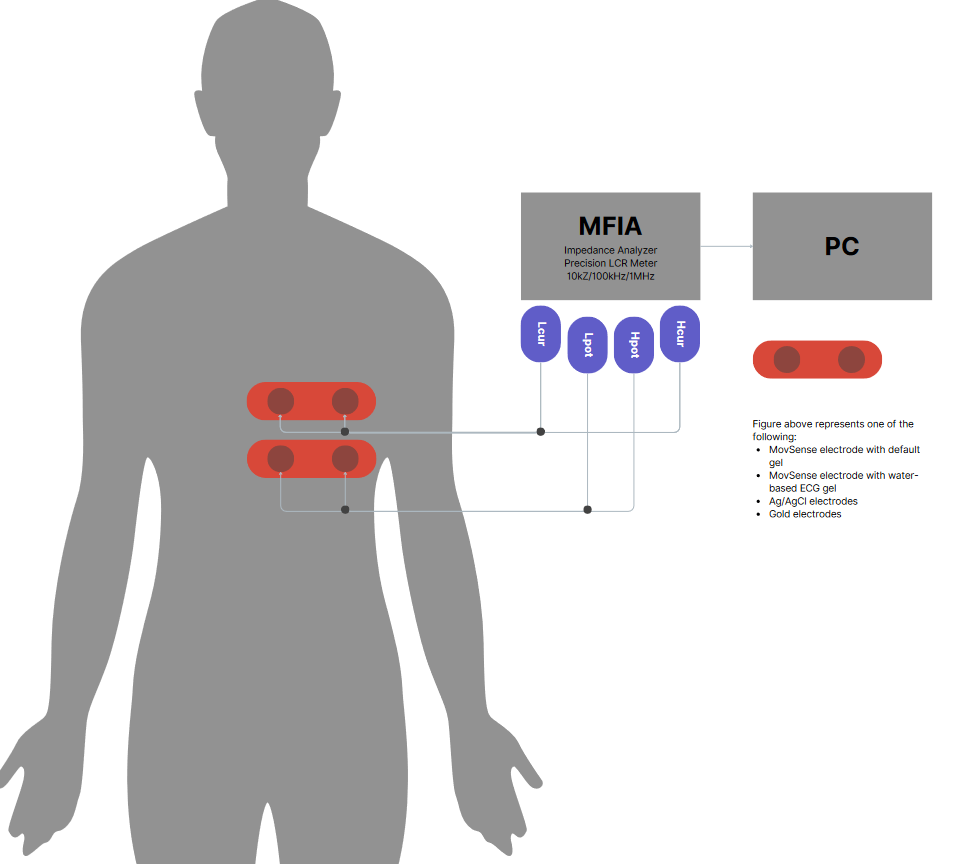
\includegraphics[width=0.5\textwidth]{figures/experimentSetup.png}
    \caption{Experimental setup for evaluating electrode performance in bioimpedance measurements and BCC applications.}
    \label{fig:experimental_setup}
\end{figure}

\begin{figure}
    \centering
    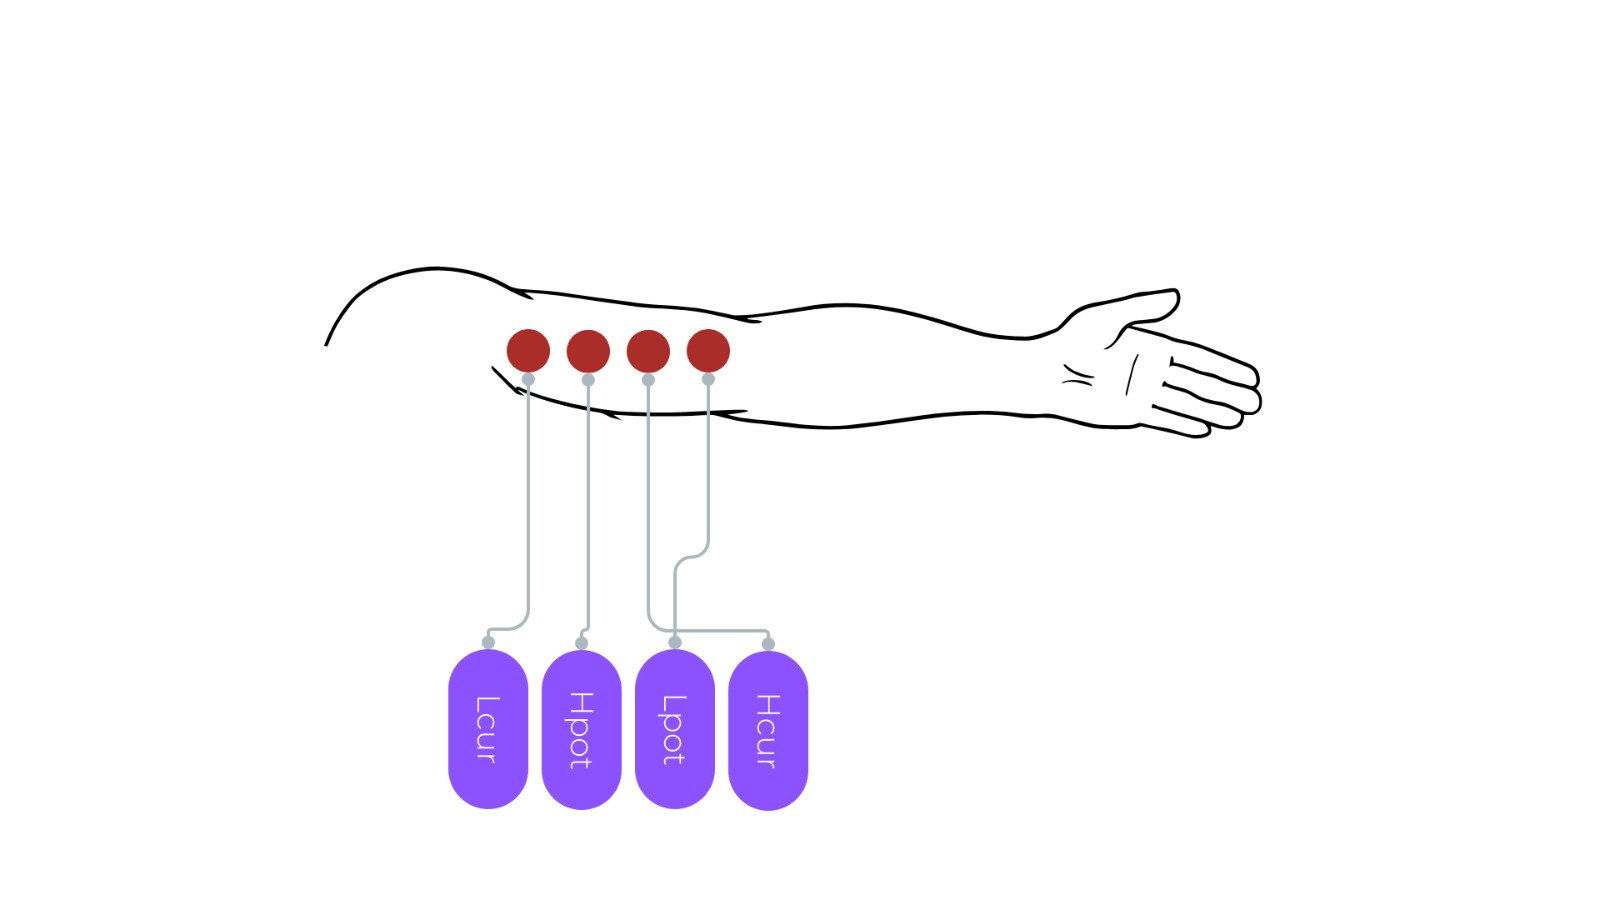
\includegraphics[width=0.5\textwidth]{figures/experimentSetup_upper_arm.jpeg}
    \caption{Experimental setup for evaluating electrode performance in bioimpedance measurements and BCC applications.}
    \label{fig:experimental_setup_upper_arm}
\end{figure}

The study employs an MFIA Impedance Analyzer for bioimpedance signal measurement and Software Defined Radios (SDRs) for evaluating BCC communication quality. Data acquisition and analysis were facilitated through custom scripts in Python, enabling the extraction of SNR, settling time, and CER metrics from the collected data.

Electrodes were tested under controlled conditions to simulate their application in BPG recording, BioZ pneumography, and BCC scenarios.

\subsection{Equipment and Materials}
\begin{itemize}
    \item Electrode Connectros that would allow to plug them to MFIA analyzer and SDR
    \item MFIA impedance analyzer
    \item Software-Defined Radios (SDRs)
    \item Ag/AgCl electrodes
    \item Gold plated electrodes
    \item EMS electrodes
\end{itemize}

\subsection{Experiment Procedure}
Each experiment will follow the steps outlined below, to be repeated for each type of electrode:

\begin{enumerate}
    \item \textbf{Preparation:} Ensure all equipment is calibrated according to the manufacturer's instructions. Prepare the subject by cleaning the skin area near the left side of the body near the last rib and upper arm for electrode placement.
    \item \textbf{Electrode Placement:} Apply one type of electrodes to the prepared skin area.
    \item \textbf{Measurement:}
    \begin{enumerate}
        \item \textbf{Heart Rate Measurement:} Instruct the subject to hold their breath. Measure the heart rate using the MFIA impedance analyzer. Record the data.
        \item \textbf{Breathing Measurement:} Without altering the electrode placement, measure the subject's breathing using the MFIA impedance analyzer. Record the data.
        
    \end{enumerate}

    \item \textbf{Repeat:} Repeat steps 1, 2 and 3 for each type of electrode and each skin area.
    \item \textbf{Electrode Placement:} Apply one pair of electrodes to chest area and another pair to the upper arm.
    \item \textbf{Data Transmission:} Utilize the SDRs to measure the data transmission capabilities of the electrodes. Record the data.
    \item \textbf{Repeat:} Repeat steps 5 and 6 for each type of electrode.
\end{enumerate}

Data were collected across static conditions to assess each electrode type's performance.




%\subsection{Evaluation Parameters}
%\notea{Duplicating with Section C...}
%\begin{itemize}
%    \item Signal-to-Noise Ratio (SNR)
%    \item Settling Time
%    \item Chip Error Rate (CER) for BCC application
%    \item Movement Artifacts Measurement Methodology
    
%For the quantification of movement artifacts, particularly in the context of BCC applications, the Chip Error Rate (CER) ratio under passive and active conditions was utilized. The formula for calculating the movement artifacts impact is given by:
%\begin{equation}
%    \text{Movement Artifacts Impact} = \frac{\text{CER\_active}}{\text{CER\_passive}}
%\end{equation}
%where CER\_active represents the chip error rate under active (movement) conditions, and CER\_passive represents the chip error rate under passive (no movement) conditions. A value greater than 1 indicates an increase in transmission errors due to movement.

%\end{itemize}


%\input{Old_sections/experimental_setup.tex}

\section{Results}

In this section, we outline the experimental outcomes from this comparison among Ag/AgCl electrodes, EMS electrodes, and gold-plated electrodes. The evaluation metrics included Signal-to-Noise Ratio (SNR) for both breathing and pulse signals, Settling Time for signal stabilization, and Chip Error Rate (CER) for Body-Coupled Communication (BCC). Instances where signal quality was insufficient for measurement are denoted by "-".

\subsection{SNR (Signal-to-Noise Ratio)}

 \textbf{Breathing (Upper Arm):} The SNR values for Ag/AgCl and EMS electrodes were 10 and 12, respectively, with gold-plated electrodes at a lower SNR of 5.
 
\textbf{Breathing (Chest):} Gold-plated electrodes significantly outperformed with an SNR of 30, against 10 for Ag/AgCl and 15 for EMS electrodes.

 \textbf{Pulse (Upper Arm):} Gold-plated electrodes exhibited a superior SNR of 1, compared to 0.5 for Ag/AgCl electrodes, with EMS electrodes' signal being too poor to measure.

 \textbf{Pulse (Chest):} The SNR for Ag/AgCl electrodes was slightly better at 1, versus 0.5 for gold-plated electrodes. The EMS electrodes' performance could not be measured.


\subsection{Settling Time}

 \textbf{Breathing (Upper Arm):} EMS electrodes demonstrated an instantaneous settling time (0 seconds), followed by gold-plated (10 seconds) and Ag/AgCl electrodes (30 seconds).
 
    \textbf{Breathing (Chest):} Gold-plated electrodes achieved the fastest settling time at 0 seconds, Ag/AgCl electrodes followed at 5 seconds, and EMS electrodes lagged at 20 seconds.
 
    \textbf{Pulse (Upper Arm):} Both Ag/AgCl and gold-plated electrodes registered a settling time of 2 seconds. EMS electrodes' quality was unmeasurable.

 \textbf{Pulse (Chest):} Settling time for gold-plated electrodes was recorded at 5 seconds, outperforming Ag/AgCl electrodes which stood at 7 seconds. EMS electrodes' signal was again unmeasurable.


\subsection{CER (Chip Error Rate) in BCC}

The Chip Error Rate for Body-Coupled Communication was found to be lowest for Ag/AgCl electrodes at 3.30\%, followed by EMS at 5.20\%, and gold-plated electrodes at 5.50\%.

These experimental insights depict a nuanced landscape of electrode performance, where no single type consistently excels across all metrics. Notably, gold-plated electrodes demonstrate superior capability in specific scenarios, particularly in SNR for chest breathing signals and the settling time for breathing signals, highlighting their application-specific advantages. However, their performance varied across the board, emphasizing the importance of tailored electrode choice based on precise application needs. The EMS electrodes faced challenges in reliable signal acquisition for some metrics, indicating their limitations in the tested scenarios.


\begin{table}[!ht]
    \centering
    \caption{Summary of experimental results for electrode performance across different metrics and scenarios.}
    \begin{tabular}{|l|l|l|l|}
    \hline
        Metric & Ag/AgCl & EMS & Gold \\ \hline
        SNR - Breathing - Upper Arm & 10 & 12 & 5 \\ \hline
        SNR - Breathing - Chest & 10 & 15 & 30 \\ \hline
        Settling Time - Breathing - Upper Arm & 30s & 0s & 10s \\ \hline
        Settling Time - Breathing - Chest & 5s & 20s & 0s \\ \hline
        SNR - Pulse - Upper Arm & 0.5 & - & 1 \\ \hline
        SNR - Pulse - Chest & 1 & - & 0.5 \\ \hline
        Settling Time - Pulse - Upper Arm & 2s & - & 2s \\ \hline
        Settling Time - Pulse - Chest & 7s & - & 5s \\ \hline
        CER - BCC & 3.30\% & 5.20\% & 5.50\% \\ \hline
    \end{tabular}
    
\end{table}
%\subsection{Movement Artifacts Evaluation}
%\section{Discussion}
%\subsection{Pulse Measurement Scenario Analysis}
%The pulse measurement scenario offers insightful observations into the comparative performance of Ag/AgCl electrodes, EMS electrodes, and gold-plated electrodes. This analysis is pivotal for understanding the implications of electrode choice in applications requiring precise cardiovascular monitoring.
%\textbf{Signal-to-Noise Ratio (SNR):} The SNR is a critical factor in assessing the quality of the pulse signal captured by the electrodes. This results indicate that gold-plated electrodes tend to perform better on the upper arm with an SNR of 1, compared to 0.5 for Ag/AgCl electrodes. This suggests that gold-plated electrodes may provide clearer signal quality in upper arm pulse measurements, which is essential for accurate heart rate monitoring. However, in chest measurements, Ag/AgCl electrodes slightly outperformed gold-plated ones (SNR of 1 vs. 0.5), indicating that electrode placement and the specific monitoring site play a significant role in signal clarity. The absence of data for EMS electrodes in this scenario due to unmeasurable signal quality underscores the challenges that certain electrode types may face in specific physiological monitoring contexts.
%\textbf{Settling Time:} The rapid stabilization of the signal, as denoted by the settling time, is crucial for timely and efficient pulse monitoring. Both Ag/AgCl and gold-plated electrodes showed a settling time of 2 seconds on the upper arm, indicating a quick adaptation to the physiological signal. This quick settling time is advantageous in scenarios where immediate signal acquisition is necessary, such as in acute care settings. For chest measurements, gold-plated electrodes demonstrated a slightly better settling time (5 seconds) compared to Ag/AgCl electrodes (7 seconds), suggesting that for chest-based pulse measurements, gold-plated electrodes might be slightly more efficient in achieving signal stability.
%\textbf{Application Implications:} The choice between Ag/AgCl and gold-plated electrodes for pulse measurements should consider both the monitoring location and the specific requirements of the application. For upper arm measurements where higher SNR is a priority, gold-plated electrodes appear to offer an advantage. Conversely, for chest measurements, the choice may depend on the balance between the need for slightly higher SNR (favoring Ag/AgCl electrodes) and faster settling times (favoring gold-plated electrodes). The unavailability of data for EMS electrodes in pulse measurements suggests a limitation in their utility for reliable cardiovascular monitoring, highlighting the need for further research into electrode designs that can accommodate a broader range of measurement scenarios.
%Overall, the pulse measurement scenario underscores the nuanced trade-offs between electrode types, with no single electrode type emerging as universally superior across all metrics. This analysis illustrates the importance of context in electrode selection, where specific application needs and measurement site characteristics should guide the choice of electrodes. Further research into optimizing electrode materials and designs for specific physiological signals and monitoring locations could significantly enhance the efficacy and reliability of biomedical monitoring technologies.
%This section delves into the comparative analysis of BioZ pneumography measurements, focusing on the performance of Ag/AgCl electrodes, EMS electrodes, and gold-plated electrodes across different scenarios. Pneumography, the process of recording breathing patterns, is crucial in both clinical settings and wearable health technology. The efficacy of this measurement largely depends on the quality of the electrodes used for signal acquisition.
%\subsection{BioZ Pneumography Measurement Analysis}
%The signal-to-noise ratio (SNR) and settling time serve as critical parameters in evaluating the performance of electrodes in BioZ pneumography measurements. These metrics directly impact the reliability and accuracy of respiratory rate monitoring, a vital sign that is indicative of numerous health conditions.
%\subsubsection{Signal-to-Noise Ratio (SNR)}
%\textbf{Upper Arm vs. Chest Measurements:} The experimental results highlight a stark difference in performance among the electrode types when used for pneumography. Notably, gold-plated electrodes exhibited superior SNR in chest measurements with a value of 30, significantly outperforming both Ag/AgCl and EMS electrodes. This suggests that gold-plated electrodes are more adept at capturing the subtle changes in bioimpedance caused by breathing at the chest level, attributed to their enhanced conductivity and biocompatibility. However, in the upper arm scenario, the performance of gold-plated electrodes was the lowest with an SNR of 5, which could be due to the reduced impact of thoracic movement on bioimpedance at this location.
%\textbf{Implications for Clinical and Wearable Applications:} The high SNR of gold-plated electrodes in chest measurements underlines their potential in applications requiring high precision in respiratory rate monitoring, such as in patients with respiratory disorders or for sleep quality studies. Conversely, the lower SNR observed in upper arm measurements across all electrode types suggests a potential limitation in scenarios where chest placement is not feasible.
%\subsubsection{Settling Time}
%\textbf{Rapid Signal Acquisition:} The settling time—how quickly a stable signal is obtained—was found to be minimal for gold-plated electrodes in chest measurements (0 seconds), indicating their suitability for scenarios requiring immediate data collection, such as emergency medical services or real-time health monitoring systems.
%\textbf{Upper Arm Measurements:} In contrast, for upper arm measurements, EMS electrodes demonstrated an immediate settling time of 0 seconds, suggesting that despite their lower SNR, they may offer advantages in scenarios where rapid setup and less precise respiratory monitoring are acceptable.
%\subsection{Overall Evaluation}
%The evaluation of BioZ pneumography measurements underscores the importance of selecting the appropriate electrode type based on the specific requirements of the application. Gold-plated electrodes, with their exceptional performance in chest measurements, emerge as a preferable choice for detailed respiratory analysis. However, the context of the measurement, including the location (chest vs. upper arm) and the need for rapid signal acquisition, plays a crucial role in determining the most suitable electrode type.
%In conclusion, this analysis reveals the nuanced trade-offs between electrode types in BioZ pneumography measurements. Future research should further explore these dynamics, potentially leading to the development of specialized electrodes tailored to specific measurement scenarios.
%\subsection{BCC Application Analysis}
%In evaluating the efficacy of electrodes for Body-Coupled Communication (BCC), Chip Error Rate (CER) serves as a pivotal metric. BCC leverages the human body as a medium for signal transmission, a novel approach that underpins many emerging applications in health monitoring and data transfer. The CER, which measures the rate of errors in the communication channel, directly impacts the reliability and efficiency of these applications.
%\subsubsection{Chip Error Rate (CER)}
%\textbf{Comparative Analysis:} The experimental findings indicated that Ag/AgCl electrodes exhibited the lowest CER at 3.30\%, followed by EMS electrodes at 5.20\%, and gold-plated electrodes at 5.50\%. This suggests that Ag/AgCl electrodes provide a more stable and reliable channel for body-coupled communication, likely due to their effective impedance matching with human skin, which is critical for minimizing signal loss and reflections.
%\textbf{Implications for BCC Applications:} The lower CER of Ag/AgCl electrodes highlights their potential in applications where high data integrity and minimal transmission errors are paramount. These scenarios include wearable health technologies that rely on the seamless exchange of physiological data between devices or remote monitoring systems where accuracy and reliability are crucial.
%However, the relatively higher CER observed with gold-plated and EMS electrodes does not necessarily preclude their use in BCC applications. The selection of electrodes must also consider factors such as biocompatibility, durability, and the specific communication requirements of the application. For instance, gold-plated electrodes, despite their higher CER, might still be preferred in long-term monitoring applications due to their superior biocompatibility and resistance to corrosion. 
%\subsubsection{Strategic Considerations for Electrode Selection in BCC}
%The nuanced performance differences among electrode types in BCC applications underscore the importance of strategic electrode selection. Developers and researchers should weigh the trade-offs between CER, biocompatibility, durability, and economic factors to determine the most suitable electrode type for their specific application. Moreover, the evolving landscape of BCC technology may necessitate ongoing evaluation as new electrode materials and designs emerge. As to BCC technology relies on long-term wearability and user comfort, these factors are equally important in electrode selection. In glance of the results and very insignificant diferences in CERs, the choice of electrode type for BCC applications may fall to reusable EMS and gold-plated electrodes, as they offer a balance between performance and durability.
%In conclusion, this analysis of BCC applications reveals a complex interplay between electrode material properties and communication performance. While Ag/AgCl electrodes currently offer the lowest CER, the broader context of application requirements must guide the final electrode selection. Future advancements in electrode technology and BCC methodologies hold the promise of further enhancing the efficacy of body-coupled communication in healthcare and beyond.
%\subsection{Movement Artifacts Across Scenarios}

\section{Discussion}

This comprehensive investigation into Ag/AgCl, EMS, and gold-plated electrodes has yielded nuanced insights into their performance across bioimpedance measurements and Body-Coupled Communication (BCC), underscoring the complex interplay between material properties and application-specific requirements. This discussion seeks to contextualize this findings within the broader landscape of biomedical engineering and wearable technology, drawing connections to existing literature and highlighting potential avenues for future research.

\subsection{Comparative Analysis of Electrode Performance}

The differential performance of Ag/AgCl, EMS, and gold-plated electrodes across various metrics—such as Signal-to-Noise Ratio (SNR), Settling Time, and Chip Error Rate (CER)—emphasizes the critical role of electrode material and design in biomedical applications. Gold-plated electrodes demonstrated superior SNR in certain scenarios, aligning with findings by Zhao et al. \cite{Zhao2018Fabrication}, who highlighted the excellent electrical conductivity and minimal signal distortion of gold as a material. However, this study extends these observations by comparing gold-plated electrodes' performance not just on electrical properties but also on their application in real-world biomedical monitoring scenarios, offering a comprehensive view of their utility.

\subsection{Implications for Wearable Technology and Patient Monitoring}

The variation in electrode performance across different applications—particularly in the context of wearable technology and patient monitoring—highlights the importance of selecting the right electrode type based on specific use-case requirements. For instance, the superior performance of gold-plated electrodes in terms of SNR for chest breathing measurements suggests their suitability for respiratory monitoring applications, which is crucial for managing conditions such as asthma or chronic obstructive pulmonary disease (COPD). This finding aligns with recent advancements in wearable respiratory monitoring technologies, which emphasize the need for high fidelity in signal capture \cite{rabbani2023low}.

\subsection{BioZ and BCC: Bridging the Gap Between Diagnosis and Communication}

This study's focus on both BioZ and BCC technologies reflects an emerging trend in the field: the integration of diagnostic and communication capabilities within a single wearable platform. The lower CER observed with Ag/AgCl electrodes in BCC applications suggests their potential for enhancing the reliability of data transmission through the human body. This capability is pivotal for the next generation of wearable devices that not only monitor health metrics but also communicate these data securely to healthcare providers or other devices. The integration challenges and opportunities highlighted by this findings suggest a fertile ground for innovation, echoing the sentiment of recent studies that call for a unified approach to wearable health technology development \cite{zaira2023prediction}.

\subsection{Future Research Directions}

Looking ahead, several areas warrant further investigation to build on this findings. The development of new electrode materials that combine the biocompatibility and durability of gold with the cost-effectiveness and environmental sustainability of Ag/AgCl represents a significant research opportunity. Additionally, exploring the impact of electrode size, shape, and placement on both diagnostic accuracy and wearer comfort could yield valuable insights for the design of next-generation wearable devices. Finally, advancing the capabilities of BCC technology, particularly in terms of reducing CER and enhancing data transmission rates, remains a critical challenge for the field.

\subsection{Concluding Remarks}

In conclusion, this study contributes to a deeper understanding of the critical factors influencing electrode selection in biomedical applications, bridging the gap between material science and wearable technology development. By offering a comprehensive comparison of Ag/AgCl, EMS, and gold-plated electrodes, we highlight the nuanced trade-offs that must be navigated to optimize the performance of bioimpedance measurements and body-coupled communication systems. This work lays the groundwork for future research aimed at enhancing the efficacy, reliability, and user-friendliness of non-invasive diagnostic and communication technologies in healthcare.





%\section{Conclusion}
%This study embarked on a comprehensive evaluation of three types of electrodes - Ag/AgCl, EMS, and gold-plated - across a range of biomedical applications, including bioimpedance measurements and Body-Coupled Communication (BCC). Through rigorous testing, we have derived critical insights into the performance metrics of these electrodes, notably in terms of Signal-to-Noise Ratio (SNR), Settling Time, and Chip Error Rate (CER).
%\subsection{Summary of Findings}
%This results indicate that for short term measurements the most suitable electrodes are the Classical Ag/AgCl Disposable Electrodes. However, for long term measurements, the gold-plated electrodes shows that their benifits are much valuable than inconvinience of custom electrode manufacturing. The performance of EMS electrodes varied, showing promise in certain scenarios but limited by unmeasurable signal quality in pulse measurements.
%\subsection{Future Research Directions}
%Future research should focus on several key areas:
%\begin{enumerate}
%    \item Developing electrode materials and designs that offer a balanced performance across a wider range of biomedical applications.
%    \item Exploring the impact of electrode size, shape, and placement on measurement accuracy and user comfort in bioimpedance and BCC applications.
%    \item Investigating the long-term durability and biocompatibility of electrodes, particularly for wearable devices intended for continuous health monitoring.
%    \item Advancing BCC technology to improve data transmission efficiency, reduce CER, and expand its applicability in next-generation wearable health systems.
%    \item Performe same tests with unprepared skin to see how the results differ.
%\end{enumerate}
%In conclusion, this study provides valuable insights into the comparative performance of different electrode types in bioimpedance measurements and BCC applications. By highlighting the strengths and limitations of Ag/AgCl, EMS, and gold-plated electrodes, we contribute to the informed selection of electrode materials in the development of advanced biomedical devices. The pursuit of optimized electrode solutions remains a critical endeavor as we advance towards more accurate, reliable, and user-friendly non-invasive diagnostic and communication technologies in healthcare.
% Add the References section as per your formatting guideline.

\section{Conclusion}

This rigorous examination of Ag/AgCl, EMS, and gold-plated electrodes within the realms of bioimpedance measurements and Body-Coupled Communication (BCC) has unveiled intricate insights into their performance, applicability, and impact on future healthcare technologies. This research not only delineates the technical attributes of these electrodes but also emphasizes their potential in revolutionizing patient care through enhanced diagnostic and communication capabilities.

\subsection{Key Findings and Implications}

The study's findings reveal a distinct performance landscape where each electrode type exhibits unique strengths and limitations across different biomedical applications. Ag/AgCl electrodes, with their lower Chip Error Rate (CER), emerge as a preferred choice for BCC applications, ensuring reliable data transmission through the human body. This characteristic is pivotal for wearable technologies that necessitate secure and efficient communication of health data. On the other hand, gold-plated electrodes showcase superior Signal-to-Noise Ratio (SNR) in specific scenarios, such as chest-based respiratory monitoring, highlighting their potential for applications requiring high precision in signal capture. The EMS electrodes, with their instant settling time, offer an intriguing balance between performance and user comfort, suggesting their suitability for long-term monitoring applications where rapid signal stabilization is crucial.

These findings bear significant implications for the design and development of next-generation wearable healthcare devices. By selecting the appropriate electrode type based on the specific needs of the application, device manufacturers can enhance the accuracy, reliability, and user experience of wearable diagnostics and communication systems. This, in turn, can lead to more personalized and effective patient care, empowering individuals to manage their health proactively.

\subsection{Future Research Directions}

Looking forward, the study opens several avenues for further research aimed at overcoming the current limitations and unlocking the full potential of electrode technologies in healthcare. A key area of focus is the development of new electrode materials and configurations that marry the best attributes of the examined electrode types, such as the biocompatibility and durability of gold with the cost-effectiveness of Ag/AgCl. Investigating the impact of electrode size, shape, and placement on measurement accuracy and wearer comfort will also be critical for optimizing the design of wearable devices.

Moreover, advancing the capabilities of Body-Coupled Communication technology to improve data transmission efficiency and reduce error rates remains a crucial challenge. Addressing these issues can significantly enhance the functionality and reliability of wearable health systems, making them more adaptable to diverse healthcare applications.

\subsection{Concluding Reflections}

In sum, this comparative study of Ag/AgCl, EMS, and gold-plated electrodes provides valuable insights into the complex considerations involved in electrode selection for biomedical applications. By highlighting the nuanced trade-offs between technical performance, user comfort, and environmental sustainability, this research contributes to the informed development of advanced wearable health technologies. As we continue to explore and innovate in this space, the pursuit of optimized electrode solutions will play a critical role in shaping the future of non-invasive diagnostics and communication in healthcare, ultimately leading to better health outcomes and quality of life for patients worldwide.





\bibliographystyle{IEEEtran}
\bibliography{IEEEabrv,bibliography.bib}

\end{document}